\documentclass[11pt]{article}
\usepackage{../shared/hanzocover}
\usepackage[utf8]{inputenc}
\usepackage[T1]{fontenc}
\usepackage{amsmath,amssymb}
\usepackage{graphicx}
\usepackage{booktabs}
\usepackage{xcolor}
\usepackage{listings}
\input{../shared/lstlang}
\usepackage{tikz}
\usetikzlibrary{shapes,arrows.meta,positioning,fit,backgrounds,calc}
\usepackage[hidelinks]{hyperref}

\definecolor{codegreen}{rgb}{0,0.6,0}
\definecolor{codegray}{rgb}{0.5,0.5,0.5}
\definecolor{codepurple}{rgb}{0.58,0,0.82}
\definecolor{backcolour}{rgb}{0.96,0.96,0.94}
\definecolor{hzblue}{rgb}{0.12,0.30,0.55}
\definecolor{hzslate}{rgb}{0.22,0.25,0.30}
\definecolor{hzgreen}{rgb}{0.10,0.45,0.25}
\definecolor{hzred}{rgb}{0.60,0.16,0.16}

\lstdefinestyle{mystyle}{
    backgroundcolor=\color{backcolour},
    commentstyle=\color{codegreen},
    keywordstyle=\color{codepurple},
    numberstyle=\tiny\color{codegray},
    stringstyle=\color{codegreen},
    basicstyle=\ttfamily\footnotesize,
    breakatwhitespace=false,
    breaklines=true,
    captionpos=b,
    keepspaces=true,
    numbers=none,
    showspaces=false,
    showstringspaces=false,
    showtabs=false,
    tabsize=2,
    frame=single,
    rulecolor=\color{codegray}
}
\lstset{style=mystyle}

\title{Hanzo Router: Memory-Aware, Local-First LLM Routing with a Learned SLO-Constrained Policy}
\author{Hanzo AI Research\thanks{Corresponding author: research@hanzo.ai} \\
    \textit{Hanzo Industries Inc (Techstars '17)} \\
    Los Angeles, California \\
    \texttt{https://hanzo.ai}}
\date{Hanzo Research}

\begin{document}

\hanzocoverpage

\twocolumn[
  \begin{@twocolumnfalse}
  \maketitle
  \begin{abstract}
  \noindent
  Frontier language models are priced for their hardest queries, but a
  production request stream is dominated by its easiest ones: short chats,
  classification, formatting, and boilerplate code that a small local model
  answers as well as a frontier API. Paying the frontier price on every token
  is the single largest avoidable cost in an LLM product. We describe
  \emph{Hanzo Router}, the request router that \texttt{hanzo-node} uses to place
  each request across a swappable pool of local and cloud models. The design
  decomplects \emph{mechanism} from \emph{brain}. The mechanism
  (\texttt{hanzo-router}) is pure logic over value inputs: a model registry, a
  memory snapshot, the set of already-loaded models, and a per-request
  service-level objective; it prefers, in order, reusing a model already
  resident (zero marginal cost), loading a local model that fits available
  memory, then the cheapest usable cloud model. The brain is a swappable policy
  behind a one-method seam: a rule-based cold-start policy, a learned bilinear
  utility with per-user online adaptation (\texttt{enso}), or a small trainable
  routing encoder (\texttt{zen-router}). We give the SLO-constrained objective
  the learned policy optimizes, $\mathrm{quality}-\lambda\,\mathrm{cost}-\mu\,\mathrm{latency}$
  under hard feasibility ceilings; the memory-aware fit check that makes
  local-first placement deterministic and unit-testable; the online LinUCB loop
  that personalizes routing from observed rewards; and a usage-plane signal that
  biases routing away from providers near their rate limits. We do not claim a
  measured benchmark saving. Instead we give a transparent, itemized cost model
  that goes beyond API token prices: for a mixed workload whose simple traffic
  is served locally for the price of electricity (not a rented GPU) and whose
  medium traffic drops to a cheap cloud tier, the arithmetic yields roughly a
  90\% reduction in total AI spend---token cost, avoided cloud-GPU rental,
  consolidated per-seat subscriptions, and rate-limit overage---in line with
  the published routing and cascade literature.
  \end{abstract}
  \vspace{1.5em}
  \end{@twocolumnfalse}
]

\section{Introduction}
\label{sec:intro}

A frontier language model is priced for the worst case. Its per-token rate has
to cover the queries that genuinely need a trillion-parameter model: multi-step
reasoning, long-context synthesis, hard code generation. But the request stream
of a deployed product does not look like that benchmark. It is dominated by
easy traffic: a one-line clarification, a yes/no classification, a JSON reformat,
an autocomplete, a boilerplate function. On that traffic a 4B model running on a
laptop is indistinguishable from a frontier API to the end user, and it costs
only electricity per token---about two orders of magnitude below frontier API
pricing (\S\ref{sec:cost})---on hardware already paid for.

Routing every request to the frontier model therefore spends the frontier price
on a stream whose median query does not need it. This is the single largest
avoidable line item in an LLM product's bill, and it is avoidable precisely
because the mismatch is structural: the price is set by the tail, the volume is
in the head. A router that sends each request to the cheapest model that can
still serve it converts that structural mismatch into a cost saving, without a
user-visible quality regression, provided it can tell the two kinds of request
apart and provided it has somewhere cheap to send the easy ones.

This paper describes the router Hanzo runs in production, \texttt{hanzo-router},
and its learned policy \texttt{enso}. The contribution is not a new model; it is
an architecture that makes cheap-when-you-can, frontier-when-you-must routing a
first-class, testable, learnable component of the serving stack. We make four
claims. First, the routing \emph{mechanism} should be pure logic over value
inputs, with no hardware access of its own, so that placement is deterministic
and unit-testable (\S\ref{sec:mechanism}). Second, local-first placement is a
memory-fit problem: given a snapshot of available memory and the set of models
already resident, the router reuses, loads, or falls through to cloud by a
single ordered walk of preferences (\S\ref{sec:mechanism}). Third, the
\emph{policy} that ranks models is a swappable brain behind a one-method seam,
so a rule guess, a learned bilinear utility, and a trainable encoder are
interchangeable and compose (\S\ref{sec:brain}, \S\ref{sec:learning}). Fourth,
the saving is real but must be stated honestly: we give a transparent cost model
(\S\ref{sec:cost}) rather than a fabricated benchmark, and anchor the magnitude
in the published routing literature (\S\ref{sec:related}).

\section{The Mechanism: Memory-Aware, Local-First Placement}
\label{sec:mechanism}

The mechanism is the crate \texttt{hanzo-router}. It is deliberately dumb about
hardware and clever about values. Following the Rich Hickey discipline of
separating a decision from the place it runs~\cite{hickey_simple},
\texttt{hanzo-node} gathers the facts the decision needs into plain values and
hands them to a pure function; the router touches no device and opens no socket,
so the same inputs always produce the same decision and every path is a unit
test.

\begin{figure}[t]
\centering
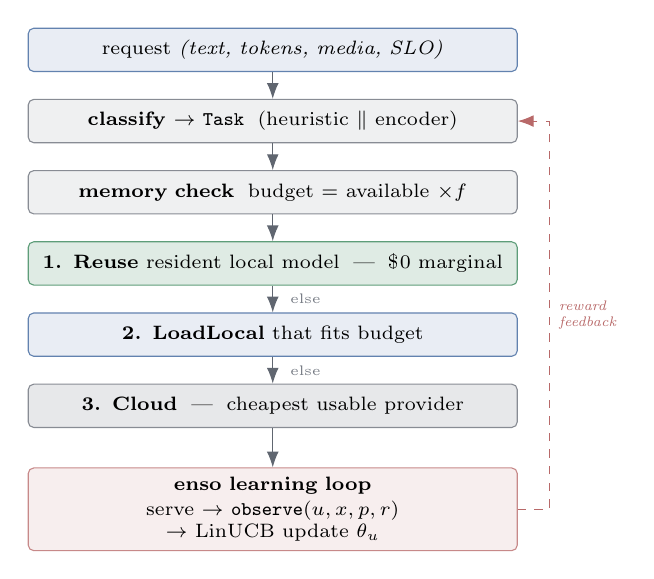
\begin{tikzpicture}[
  font=\scriptsize,
  node distance=3.4mm,
  box/.style={draw, rounded corners=2pt, align=center, minimum height=5.5mm,
              inner xsep=3pt, text width=60mm},
  stage/.style={box, fill=hzslate!8, draw=hzslate!60},
  reuse/.style={box, fill=hzgreen!14, draw=hzgreen!70},
  load/.style={box, fill=hzblue!10, draw=hzblue!70},
  cloud/.style={box, fill=hzslate!12, draw=hzslate!60},
  learn/.style={box, fill=hzred!8, draw=hzred!55},
  arr/.style={-{Latex[length=2mm]}, hzslate!80, line width=0.4pt}
]

\node[stage, fill=hzblue!10, draw=hzblue!70] (req)
  {request \textit{(text, tokens, media, SLO)}};
\node[stage, below=of req] (cls)
  {\textbf{classify} $\rightarrow$ \texttt{Task}\; (heuristic $\parallel$ encoder)};
\node[stage, below=of cls] (mem)
  {\textbf{memory check}\; budget $=$ available $\times f$};

\node[reuse, below=of mem] (reuse)
  {\textbf{1. Reuse} resident local model \;---\; \$0 marginal};
\node[load, below=of reuse] (load)
  {\textbf{2. LoadLocal} that fits budget};
\node[cloud, below=of load] (cloud)
  {\textbf{3. Cloud} \;---\; cheapest usable provider};

\node[learn, below=5mm of cloud] (loop)
  {\textbf{enso learning loop}\\[1pt]
   serve $\rightarrow$ \texttt{observe}$(u,x,p,r)$ $\rightarrow$ LinUCB update $\theta_u$};

\draw[arr] (req) -- (cls);
\draw[arr] (cls) -- (mem);
\draw[arr] (mem) -- (reuse);
\draw[arr] (reuse) -- (load) node[midway, right=1mm, hzslate!70, font=\tiny] {else};
\draw[arr] (load) -- (cloud) node[midway, right=1mm, hzslate!70, font=\tiny] {else};
\draw[arr] (cloud) -- (loop);
\draw[arr, dashed, hzred!70] (loop.east) -- ++(4mm,0) |- (cls.east)
  node[pos=0.25, right, hzred!70, font=\tiny\itshape, align=left] {reward\\feedback};

\end{tikzpicture}
\caption{The router decision flow. A request is classified to a task, checked
against the memory budget, and placed by the ordered walk: reuse a resident
local model (zero marginal cost), else load a local model that fits, else fall
through to the cheapest usable cloud model. The learned policy (\texttt{enso})
closes the loop---each served request yields a reward that updates the per-user
LinUCB weights and, through them, future routing.}
\label{fig:decision}
\end{figure}


\subsection{The pool as a registry of value rows}

Every servable model is one \texttt{ModelCard}: a canonical id, a
\texttt{Backend} that is either \texttt{Local\{est\_bytes\}} (served by a local
\texttt{hanzo-engine}, with the resident footprint the router fits against
memory) or \texttt{Cloud\{provider\}}; the set of \texttt{Task}s the model is
preferred for; its maximum context; a vision flag; and a relative
\texttt{cost\_per\_1k}. Adding a model is adding a row. Tasks are a coarse
taxonomy---\texttt{Code}, \texttt{Reasoning}, \texttt{Math}, \texttt{Creative},
\texttt{Vision}, \texttt{LongContext}, \texttt{CheapChat}, \texttt{General}---used
only to rank quality within a modality pool; modality (text, vision, image,
audio, video) selects the pool itself. The two axes are orthogonal, so one
router serves chat, vision, and media generation by matching pools.

A request is classified to a task by a \texttt{Classifier}. The default
\texttt{Heuristic} is keyword-, length-, and media-based: fenced code or words
like ``bug'' and ``refactor'' route to \texttt{Code}; ``prove'', ``theorem'',
``integral'' route to \texttt{Math}; a prompt over 32k tokens is
\texttt{LongContext}; a prompt of a handful of tokens is \texttt{CheapChat};
everything else is \texttt{General}. The heuristic is a seam, not a commitment:
the \texttt{Classifier} trait lets a learned model produce the same
\texttt{Task} value without the policy changing, which is exactly where
\texttt{zen-router} (\S\ref{sec:brain}) plugs in.

\subsection{Memory as a value, and the fit check}

The one physical fact the router needs is how much memory it can spend. That,
too, is a value: a \texttt{MemSnapshot} carrying \texttt{available\_bytes},
\texttt{total\_bytes}, and a \texttt{unified} flag, filled by \texttt{hanzo-node}
from the same \texttt{MemoryUsage}/\texttt{DeviceMemory} signal the engine's
auto device-mapper reads. The usable budget for resident weights is a fraction
of available memory,
\begin{equation}
\mathrm{budget} = \mathrm{available\_bytes}\times f,
\end{equation}
and a local model of footprint $b$ fits iff $b \le \mathrm{budget}$. The default
fraction mirrors the engine's own policy: $f=0.85$ on unified-memory devices
(Apple Silicon, GB10/DGX-Spark, Strix Halo), where weights, KV cache, and
activations share one pool, and $f=0.7$ on a discrete GPU, where a reserve is
kept for activations and KV. The operator can override $f$; nothing else about
the fit check is tunable, because nothing else needs to be.

\subsection{The ordered walk}

Given a classified task, the registry, a memory snapshot, and the set of
currently-running model ids, the decision (\texttt{Policy::select}) is a single
ordered walk of the task's candidate models. Candidates are assembled in
preference order: the policy's explicit \texttt{prefer[task]} list first, then
models that explicitly advertise the task, then \texttt{General} catch-all
models last---so a task specialist outranks a generalist even if the specialist
is in the cloud. The walk then applies one rule:

\begin{enumerate}
\item \textbf{Reuse.} If any usable candidate is local and already resident in a
connectable engine, serve it. This is the zero-marginal-cost path and it wins
outright, even over a smaller model that would also fit, because a load already
paid for is cheaper than any load not yet paid for.
\item \textbf{Load local, or fall through.} Otherwise walk the candidates in
preference order. The first that is a local model whose footprint \emph{fits}
available memory is loaded and served; the first that is a usable cloud model is
routed to. A higher-preference local model that does not fit is skipped, and the
walk falls through to the next preference---which may be cloud. This is
literally ``run it locally if the RAM is there, else the next best wherever it
is.''
\item \textbf{NoFit.} If nothing is resident, nothing local fits, and no cloud
model is usable, the router returns \texttt{NoFit} and the caller errors rather
than silently degrading.
\end{enumerate}

Usability filters a candidate out before it is considered: a vision request
requires \texttt{vision}; a request needing $k$ tokens of context requires
$\texttt{max\_context}\ge k$; and a cloud model priced above the policy's
\texttt{cost\_ceiling} is refused. The whole of \texttt{select} is a few dozen
lines and every branch above is a named test in the crate---reuse-over-reload,
fall-to-cloud-when-local-does-not-fit, vision-requires-a-vision-model,
cheap-chat-prefers-cheapest-cloud, and no-fit.

\section{The Brain: A Swappable Policy Behind One Seam}
\label{sec:brain}

Placement is mechanism; \emph{which model is best for this request and this
user} is policy, and policy is where learning belongs. The two are joined by a
single trait, \texttt{RoutePolicy}, with one method: given a request, the user
it is for, an SLO, and the registry, return a \texttt{Route}---a model, an effort
\texttt{Level} (\texttt{Fast}/\texttt{Balanced}/\texttt{Max}), a modality, and a
confidence. Everything the mechanism owns---the registry, the SLO gate,
placement, dispatch---sits on one side of the seam; everything the brain owns
sits on the other. Three brains implement the seam and interchange freely.

\paragraph{The rule-based cold-start policy.} \texttt{hanzo-router}'s own
\texttt{Policy} implements \texttt{RoutePolicy}: it classifies with the
heuristic, walks candidates in preference order, and returns the first usable
one at \texttt{Balanced} with a fixed low confidence---enough to act on, low
enough that a learned policy knows it is an un-personalized guess. This is the
floor: a fresh deployment routes sensibly before any eval data exists, and any
learned brain delegates to it when it has no profiles for a pool.

\paragraph{The learned utility (\texttt{enso}).} The production brain is
\texttt{enso}, six orthogonal pieces with one concern each: a featurizer
(request $\to$ feature vector $x$), a profile table (eval rows $p$ per
$(\text{model},\text{level},\text{modality})$), a learnable bilinear utility, a
two-tier safety guard, an SLO-constrained selector, and a learner
(\S\ref{sec:learning}). It scores every candidate profile by a bilinear form and
picks the SLO-feasible argmax, falling back to the rule policy on cold start or
an empty pool.

\paragraph{The trainable encoder (\texttt{zen-router}).} At the classifier and
featurizer seams sits an optional 0.6B routing model,
\texttt{zen-router}~\cite{zenrouter}, with task, route, and feature heads. It is
supervised from eval and usage-ledger data and refined with GRPO~\cite{grpo} on
the same objective the selector optimizes, $\mathrm{quality}-\lambda\,\mathrm{cost}-\mu\,\mathrm{latency}$.
Because it produces exactly the \texttt{Task} and feature values the existing
seams already consume, it drops in without touching the mechanism or the
selector---a learned front-end for a policy whose shape does not change.

\section{The SLO Objective and Online Adaptation}
\label{sec:learning}

\subsection{Bilinear utility}

\texttt{enso}'s model of quality is deliberately a single matrix. For a request
feature vector $x\in\mathbb{R}^{D}$ and a profile vector $p\in\mathbb{R}^{K}$,
the utility is the bilinear form
\begin{equation}
u(x,p) = x^{\top} W p, \qquad W\in\mathbb{R}^{D\times K}.
\end{equation}
With the task one-hot in $x$ and quality-by-task in $p$, $W$ learns exactly the
task-to-quality alignment routing needs, and stays one matrix an online learner
can update convexly. A richer head---an MLP over $\phi=\mathrm{vec}(xp^{\top})$,
a low-rank neural encoder---attaches at this same seam by replacing the dot with
a network, without touching any other piece; the linear head is what keeps the
online learner convex and the offline fit closed-form.

\subsection{The SLO-constrained decision}

The per-request service-level objective is a value the caller sets---the
operator's budget for \emph{this} request, distinct from the user's learned
taste. It carries hard ceilings ($\texttt{max\_latency\_ms}$,
$\texttt{max\_cost}$, $\texttt{min\_quality}$; zero disables a ceiling) and two
soft weights ($\lambda=\texttt{lambda\_cost}$, $\mu=\texttt{mu\_latency}$). Over
the profiles in the request's modality pool that satisfy the ceilings, the
selector takes
\begin{equation}
\arg\max_{p\,:\,\text{feasible}(p)}\; u(x,p) - \lambda\,\widehat{c}(p) - \mu\,\widehat{\ell}(p),
\end{equation}
where $\widehat{c}$ and $\widehat{\ell}$ are normalized cost and latency and
feasibility is
\begin{equation}
\ell(p)\le \texttt{max\_latency\_ms}\;\wedge\; c(p)\le \texttt{max\_cost}\;\wedge\; q_t(p)\ge \texttt{min\_quality}.
\end{equation}
The hard ceilings gate; the soft weights trade. A cost-saver deployment raises
$\lambda$; a latency-first deployment raises $\mu$; a quality floor is enforced,
not traded, by \texttt{min\_quality}. Confidence is the squashed margin to the
runner-up, so a close call is reported as a close call. The same
\texttt{feasible} predicate gates the learned selector and the ground-truth
oracle, so the two are compared on identical constraints.

\subsection{Online adaptation}

Offline, the base $W$ is a closed-form ridge fit~\cite{ridge} of observed eval
quality on the bilinear feature $\phi=\mathrm{vec}(xp^{\top})$. Online, each user
carries a contextual bandit---LinUCB~\cite{linucb}---whose parameter
$\theta_u$ starts at a Gaussian prior centered on the base $W$ and drifts toward
that user's taste as outcomes arrive. The serving hot path is greedy on
$\theta_u$; the exploration bonus is computed only while learning. The feedback
is one call,
\begin{equation}
\texttt{observe}(u, x, p, r),
\end{equation}
recording a reward $r$ for the chosen $(\text{model},\text{level},\text{modality})$;
the Sherman--Morrison update keeps $A^{-1}$ and $\theta_u$ current in
closed form, and $\lVert\theta_u - W\rVert$ is the readable size of a user's
personalization. Because the reward is linear in $\phi$, the LinUCB core is
realizable and converges. Research-frontier variants---a low-rank neural
$\Delta W_u$, self-adaptive expert vectors---attach at exactly this update seam
and are deliberately not faked in the shipped code.

\section{Usage-Plane Signals as Decode Masks}
\label{sec:usage}

Cost and memory are not the only constraints on placement; provider rate limits
are a third. Hanzo's usage plane (\texttt{@hanzo/usage}) tracks, per provider,
the current rate-limit window and spend against it. A snapshot of that state is
a value the router can read like any other: a provider near its requests- or
tokens-per-minute ceiling is temporarily down-weighted or removed from the
usable set, exactly as an over-budget cloud model is removed by the cost
ceiling. Framed against the learned policy, a saturating provider acts as a
decode mask over the candidate set---it does not change what the ideal model is,
it changes which models are available to serve right now---so routing degrades
gracefully around a throttled provider instead of failing requests against it.
The signal is advisory and orthogonal: it composes with the memory fit check and
the SLO gate rather than replacing either.

\section{Cost Model}
\label{sec:cost}

We do not report a measured benchmark saving, because we have not run a
controlled A/B at the scale that would make such a number honest. What we can do
is state the arithmetic transparently, so the reader can substitute their own
workload mix and prices and see the saving fall out. The saving is not a
property of any model; it is a property of the workload's task distribution
against a price schedule.

\subsection{Per-request token economics}

Take a stream of one million requests, each averaging 1{,}000 input and 300
output tokens. A frontier model priced at \$3.00 per million input tokens and
\$15.00 per million output tokens costs, per request,
$\tfrac{1000}{10^6}\!\cdot\!3.00 + \tfrac{300}{10^6}\!\cdot\!15.00 = \$0.0075$.
A cheap cloud tier priced at \$0.15/\$0.60 per million costs $\$0.00033$ per
request---about $1/23$ of the frontier rate. A local zen model served by
\texttt{hanzo-engine} carries \emph{no per-token API charge}: the marginal API
cost is \$0 (its electricity cost is a compute line, accounted separately in
\S\ref{sec:compute}). Segment the stream by what each request needs: 70\% simple
(chat, classification, formatting) $\to$ local; 20\% medium (general, routine
code) $\to$ cheap cloud; 10\% hard (reasoning, long context) $\to$ frontier.
Table~\ref{tab:cost} works the API spend.

\begin{table}[t]
\centering
\footnotesize
\setlength{\tabcolsep}{4pt}
\begin{tabular}{@{}lrlrr@{}}
\toprule
Segment & Share & Routed to & \$/req & Routed \$ \\
\midrule
Simple  & 70\% & local (zen)   & 0.00000 & 0 \\
Medium  & 20\% & cheap cloud   & 0.00033 & 66 \\
Hard    & 10\% & frontier      & 0.00750 & 750 \\
\midrule
\textbf{Routed total}  & & & & \textbf{816} \\
\textbf{All-frontier}  & 100\% & frontier & 0.00750 & \textbf{7{,}500} \\
\bottomrule
\end{tabular}
\caption{Per-token API spend per one million requests. Baseline routes
everything to the frontier model (\$7{,}500); the router serves simple traffic
locally (no per-token API charge), drops medium traffic to a cheap tier, and
reserves the frontier model for the 10\% that needs it (\$816). Prices and mix
are inputs, not measurements; substitute your own.}
\label{tab:cost}
\end{table}

The routed stream costs \$816 in API spend against \$7{,}500 all-frontier, a
$1 - 816/7500 = 89.1\%$ reduction. The ``up to 90\%'' headline is exactly this
arithmetic, and it moves with the mix as expected: at an 80/15/5 split the saving
is 94\%, and a stream with no simple traffic saves nothing. The lever is the
share of requests that do not need the frontier model, which in real assistant
and agent traffic is the majority.

\subsection{Compute cost: local is cheap, not free}
\label{sec:compute}

Serving locally is not free---it draws power on hardware that is already
amortized. A small model (0.6B--24B) on consumer hardware draws on the order of
50\,W sustained and decodes roughly 25 tokens/s, i.e. about 2\,J per token. At
the U.S.\ average residential rate of $\approx\$0.15$/kWh~\cite{eia}, a request
of $\sim$1.3k tokens costs
\begin{equation*}
\tfrac{2\,\text{J}\times 1300}{3.6\times10^6\,\text{J/kWh}}\times \$0.15 \approx \$0.0001,
\end{equation*}
about one one-hundredth of a cent, and roughly two orders of magnitude below the
frontier API's $\sim\$0.006$/1k blended. These are order-of-magnitude estimates
(device wattage, throughput, and tariff are all inputs, not measurements); the
point is that the local token bill effectively disappears and the residual cost
is the \emph{amortized hardware}, which the developer's machine already exists to
provide.

\paragraph{Versus rented GPU.} The alternative way to get zero-per-token
economics is to self-host the open model on a \emph{rented} cloud GPU. One
always-on entry-GPU instance at $\approx\$0.80$/hr is $\approx\$580$~per month; a
redundant pair doubles it. Local-first routing onto laptops and workstations the
team already owns avoids that rental entirely---the compute the organization has
already bought becomes the local tier.

\paragraph{The fleet angle.} Owned compute can be pooled. A device that
registers into Hanzo Cloud as a run-for-pay node runs the open
\texttt{hanzoai/cloud} binary and serves an organization's \texttt{/v1} traffic
through the same metering plane, turning idle compute into capacity instead of
buying more cloud~\cite{runforpay}. Served work is priced cost-plus a fixed
resell margin (25\% over measured wholesale) and metered by the commerce ledger,
and 25\% of that served revenue is paid to the OSS contributors whose code ran
it. For an organization, the practical effect is that spare capacity on the
fleet offsets cloud spend rather than sitting idle.

\subsection{Total cost of ownership: a 20-person team}
\label{sec:tco}

API tokens are one line of the bill. Table~\ref{tab:tco} totals the monthly cost
of a 20-person engineering team running the one-million-request workload above,
against the status quo of a frontier-default API plus per-seat assistant
subscriptions. Beyond tokens, three further costs move: \emph{per-seat
subscriptions} collapse when org login shares one metered account through the
usage plane instead of 20 individual seats; \emph{provider overage} disappears
when rate-limit-aware routing shifts load before a window exhausts, so no
burst/overflow tier or wasted reset credit is bought; and \emph{operations}
simplify to one metering/billing plane (BillingGate over the commerce ledger)
instead of reconciling a stack of per-provider invoices. The consolidation
itself is priced as a small platform fee on routed usage---illustratively
1\%---which we include as a cost so the total is not flattered.

\begin{table}[t]
\centering
\footnotesize
\setlength{\tabcolsep}{4pt}
\begin{tabular}{@{}lrr@{}}
\toprule
Monthly cost line (20-person team) & Status quo & Router \\
\midrule
API token spend (Table~\ref{tab:cost})        & 7{,}500 & 816 \\
Local-tier compute (electricity)               & 0       & 70  \\
Per-seat assistant subs ($20\times\$20$)       & 400     & 0   \\
Provider overage / burst tiers                 & 150     & 0   \\
Routing + metering fee (1\% of routed usage)   & 0       & 8   \\
\midrule
\textbf{Monthly total (metered bill)}          & \textbf{8{,}050} & \textbf{894} \\
\bottomrule
\end{tabular}
\caption{Total monthly AI cost for a 20-person team on the
Table~\ref{tab:cost} workload. The metered bill falls from \$8{,}050 to \$894,
an $\approx 88.9\%$ reduction. \emph{Additionally, not summed above:} to run the
local tier on a rented GPU instead of owned hardware would cost
$\approx\$580$~per month---avoided entirely by local-first placement (the status-quo
column bills frontier API, not self-hosting, so the rental is a separate avoided
alternative). All figures are labeled assumptions, not measurements.}
\label{tab:tco}
\end{table}

The metered bill drops from \$8{,}050 to \$894, an $\approx 88.9\%$ reduction,
and local-first additionally avoids the $\approx\$580$~per month a rented GPU would
cost to serve the same local tier. The headline is the same as
Table~\ref{tab:cost}'s 89.1\% because API tokens dominate the bill; the point of
the itemization is that the other lines---compute, seats, overage, ops---move in
the \emph{same} direction, so the total saving is not an artifact of token prices
alone. This is the economics the cascade and routing literature reports
(\S\ref{sec:related}); our contribution is the mechanism that realizes it
deterministically and the policy that learns where the line between ``simple''
and ``hard'' actually falls.

\section{Related Work}
\label{sec:related}

LLM routing and cascading are an active area, and the cost economics above are
consistent with its published results. FrugalGPT~\cite{frugalgpt} cascades from
cheap to expensive models with a learned scorer that decides when a cheap
answer suffices, reporting large cost reductions at matched quality. RouteLLM
learns a binary strong/weak router from preference data and reports frontier-level
quality at a fraction of the cost by sending only the queries that need it to the
strong model~\cite{routellm}. Hybrid LLM~\cite{hybridllm} routes between a small
and a large model on a quality-aware threshold, and AutoMix~\cite{automix} mixes
models with self-verification to decide escalation. Tabi~\cite{tabi} is a
multi-level inference system that serves small models first and escalates
selectively. Our objective, $\mathrm{quality}-\lambda\,\mathrm{cost}-\mu\,\mathrm{latency}$,
is the natural continuous generalization of these binary escalation rules to a
pool of many models across local and cloud backends, and the per-user LinUCB
loop~\cite{linucb} adds online personalization that cascade work generally does
not. What is distinctive here is not the routing idea but the engineering
posture: a mechanism that is pure over value inputs and memory-aware, so that
local-first placement is deterministic and testable, and a policy seam that
lets a rule, a bilinear utility, and a trainable encoder interchange without a
rewrite.

\section{Limitations}
\label{sec:limits}

The honest scope is narrow in three places. First, the profile table that the
selector ranks over is populated from real eval data when a bench's JSONL is
available and from clearly-labeled synthetic tuples otherwise; until per-pool
eval data lands, the learned policy's absolute rankings are only as good as
those synthetic profiles, which is why the rule-based cold-start policy remains
the floor. Second, aggressive downgrading risks a quality regression on requests
the classifier misjudges as simple; the \texttt{min\_quality} ceiling is the
guard---it is enforced, not traded, so a request with a quality floor is never
served by a model below it, and a misclassified-hard request is caught by the
floor rather than by the soft cost weight. Third, the cost model is arithmetic,
not a measurement: it shows the shape of the saving under stated prices and a
stated mix, and a deployment's real saving depends on its own traffic. We report
the model rather than a benchmark precisely so that the claim cannot be mistaken
for one we did not run.

\section{Conclusion}

Frontier pricing is set by the hardest query; production volume is in the
easiest. Hanzo Router turns that structural mismatch into a cost saving by
placing each request on the cheapest model that can still serve it: reuse a
resident local model for free, load a local model that fits memory, and reserve
the cloud---and the frontier model within it---for the traffic that needs it.
The mechanism is pure logic over values and memory-aware, so placement is
deterministic and unit-tested; the brain is a swappable policy behind one seam,
so a rule guess, a learned bilinear utility with online per-user adaptation, and
a trainable routing encoder interchange and compose. The SLO objective
$\mathrm{quality}-\lambda\,\mathrm{cost}-\mu\,\mathrm{latency}$ makes the
cost/quality/latency trade explicit and per-request, with hard ceilings that
gate and a quality floor that is enforced rather than bargained away. The saving
is not magic and we do not dress it as a benchmark: it is the arithmetic of not
paying the frontier price on a stream whose median request never needed it.

{\small
\bibliographystyle{plain}
\bibliography{references}
}

\end{document}
